\chapter{Racionalna števila}




%%% Ulomki in racionalna števila

    \section{Ulomki in racionalna števila}

        
            
                \textbf{Ulomek} $\dfrac{x}{y}$ je zapis, ki predstavlja zapis deljenja 
                $$x:y=\dfrac{x}{y};\quad y\neq 0\land x,y\in\mathbb{Z}.$$
                Število/izraz $x$ imenujemo \textbf{števec}, $y$ pa \textbf{imenovalec}, med njima je \textbf{ulomkova črta}.
            
                ~
            
                Ulomek $\dfrac{x}{0}$ ni definiran (nima pomena), saj z $0$ ne moremo deliti.
            
                ~
            
                \textbf{Algebrski ulomek} je ulomek, v katerem v števcu in/ali imenovalcu nastopajo algebrski izrazi.
            
                ~
            
                Vsako celo število $x\in\mathbb{Z}$ lahko zapišemo z ulomkom: $x=\dfrac{x}{1}$.
            
                ~
            
                \textbf{Ničelni ulomek} je ulomek oblike $\dfrac{0}{y}=0; y\neq 0$.
            
                ~
            
                V ulomku, kjer v števcu ali imenovalcu nastopa negativno število, upoštevamo enakost 
                $$-\dfrac{x}{y}=\dfrac{-x}{y}=\dfrac{x}{-y}.$$
            
                ~
            
                Vsakemu neničelnemu ulomku $\dfrac{x}{y}$ lahko priredimo njegovo \textbf{obratno vrednost}:
                $$\left(\dfrac{x}{y}\right)^{-1}=\dfrac{y}{x}; \quad x,y\in\mathbb{Z}\setminus\{0\}.$$
            

        


        
            \subsection*{Racionalna števila}

            
                Množica racionalnih števil $\mathbb{Q}$ je sestavljena iz vseh ulomkov (kar pomeni, da vsebuje tudi vsa naravna in cela števila).

                $$\mathbb{Q}=\left\{\frac{x}{y}; \ x\in\mathbb{Z}, y\in\mathbb{Z}\setminus\{0\}\right\}$$
            
                \begin{figure}[H]
                \centering
                \begin{tikzpicture}
                    % \clip (0,0) rectangle (14.000000,10.000000);
                    {\footnotesize
                    
                    % Drawing segment A B
                    \draw [line width=0.016cm] (1.000000,1.500000) -- (4.460000,1.500000);%
                    \draw [line width=0.016cm] (4.540000,1.500000) -- (8.000000,1.500000);%
                    
                    % Marking point 0 by circle
                    \draw [line width=0.016cm] (4.500000,1.500000) circle (0.040000);%
                    \draw (4.500000,1.500000) node [anchor=south] { $0$ };%
                    
                    
                    % Changing color 255 0 0
                    \definecolor{r255g0b0}{rgb}{1.000000,0.000000,0.000000}%
                    \color{r255g0b0}% 
                    
                    % Marking point \mathbb{Q}^+
                    \draw (6.250000,1.500000) node [anchor=south] { $\mathbb{Q}^+$ };%
                    
                    % Drawing segment B 0
                    \draw [line width=0.016cm] (8.000000,1.500000) -- (4.540000,1.500000);%
                    }

                    
                    % Changing color 0 255 0
                    \definecolor{r0g255b0}{rgb}{0.000000,1.000000,0.000000}%
                    \color{r0g255b0}% 
                    
                    % Marking point \mathbb{Q}^-
                    \draw (2.750000,1.500000) node [anchor=south] { $\mathbb{Q}^-$ };%
                    
                    % Drawing segment A 0
                    \draw [line width=0.016cm] (1.000000,1.500000) -- (4.460000,1.500000);%
                    

                    % Changing color 0 0 0
                    \definecolor{r0g0b0}{rgb}{0.000000,0.000000,0.000000}%
                    \color{r0g0b0}% 
                    
                    % Marking point \mathbb{Q}
                    \draw (1.500000,2.000000) node  { $\mathbb{Q}$ };%
                    \color{black}
                    
                    \end{tikzpicture}
                \end{figure}
                    
            

            
                Glede na predznak razdelimo racionalna števila v tri množice:
                \begin{itemize}
                    \item \textcolor{green}{množico negativnih racionalnih števil $\mathbf{\mathbb{Q}^-}$},
                    \item množico z elementom nič: $\mathbf{\{0\}}$ in
                    \item \textcolor{red}{množico pozitivnih racionalnih števil: $\mathbf{\mathbb{Q}^+}$}.
                \end{itemize}
                $$ \mathbb{Q}=\textcolor{green}{\mathbb{Q}^-}\cup\{0\}\cup\textcolor{red}{\mathbb{Q}^+} $$
            
            

            % 
            %     Množica racionalnih števil je povsod gosta, saj lahko med poljubnima racionalnima številoma vedno najdemo racionalno število (posledično je med dvema racionalnima številoma neskončno mnogo racionalnih števil).
            % 

        

        
            
                Ulomka $\dfrac{x}{y}$ in $\dfrac{z}{w}$ sta enaka/enakovredna natanko takrat, ko je $xz=wy$; $y,z\neq 0$.
                $$\dfrac{x}{y}=\dfrac{w}{z}\Leftrightarrow xz=wy; \quad y,z\neq 0$$
            

            
                Enaka/enakovredna ulomka sta različna zapisa za isto racionalno število.
            
        ~\\



%%% naloge

        
            \begin{naloga}
                Za katere vrednosti $x$ ulomek ni definiran?
                \begin{itemize}
                    \item $\frac{x-2}{x+1}$ 
                    \item $\frac{2}{x-5}$ 
                    \item $\frac{x+2}{3}$ 
                    \item $\frac{13}{2x-5}$ 
                \end{itemize}
            \end{naloga}
        

        
            \begin{naloga}
                Za katere vrednosti $x$ ima ulomek vrednost enako $0$?
                \begin{itemize}
                    \item $\frac{x-2}{x+1}$ 
                    \item $\frac{2}{x-5}$ 
                    \item $\frac{x+2}{3}$ 
                    \item $\frac{13}{2x-5}$ 
                \end{itemize}
            \end{naloga}
        

        
            \begin{naloga}
                Ali imata ulomka isto vrednost?
                \begin{itemize}
                    \item $\frac{2}{3}$ in $\frac{10}{15}$ 
                    \item $\frac{-1}{2}$ in $\frac{1}{-2}$ 
                    \item $\frac{4}{5}$ in $\frac{-8}{-10}$ 
                    \item $\frac{5}{8}$ in $\frac{8}{5}$ 
                \end{itemize}
            \end{naloga}
        

        
            \begin{naloga}
                Za kateri $x$ imata ulomka isto vrednost?
                \begin{itemize}
                    \item $\frac{x+1}{2}$ in $\frac{3}{4}$ 
                    \item $\frac{4}{2x-1}$ in $\frac{1}{3}$ 
                    \item $\frac{x+1}{2}$ in $\frac{x-1}{-3}$ 
                    \item $\frac{x+1}{x-2}$ in $\frac{2}{5}$ 
                \end{itemize}
            \end{naloga}
        

        
            \begin{naloga}
                Ali ulomka predstavljata isto vrednost?
                \begin{itemize}
                    \item $\left(\frac{1}{2}\right)^{-1}$ in $-\frac{1}{2}$ 
                    \item $\left(\frac{2}{3}\right)^{-1}$ in $\frac{3}{2}$ 
                    \item $ 1\frac{3}{7}$ in $\left(\frac{7}{10}\right)^{-1}$ 
               \end{itemize}
            \end{naloga}
        

        
            \begin{naloga}
                Ali ulomka predstavljata isto vrednost?
                \begin{itemize}
                    \item $ 2\cdot\frac{3}{4}$ in $\frac{3}{2}$ 
                    \item $ 2\frac{3}{4}$ in $\frac{3}{2}$ 
                    \item $\left(1\frac{2}{5}\right)^{-1}$ in $ 1\frac{5}{2}$ 
                    \item $\left(1\frac{2}{5}\right)^{-1}$ in $\frac{5}{7}$ 
               \end{itemize}
            \end{naloga}
        

        
            \begin{naloga}
                Zapišite s celim delom oziroma z ulomkom.
                \begin{itemize}
                            \item $\frac{14}{5}$ 
                            \item $-\frac{5}{2}$ 
                            \item $\frac{4}{3}$ 
                            \item $\frac{110}{17}$ 
                            \item $ 3\frac{5}{8}$ 
                            \item $ 2\frac{9}{2}$                  
               \end{itemize}
            \end{naloga}
        

        % 
        %     \begin{naloga}
        %         Poenostavite.
        %         \begin{itemize}
        %             \item a 
        %         \end{itemize}
        %     \end{naloga}
        % 

        % 
        %     \begin{naloga}
        %         Poenostavite.
        %         \begin{itemize}
        %             \item a 
        %         \end{itemize}
        %     \end{naloga}
        % 

        %%% Razširjanje in krajšanje ulomkov

    \section{Razširjanje in krajšanje ulomkov}

        

            \subsection*{Razširjanje ulomka}
                Ulomek ohrani svojo vrednost, če števec in imenovalec pomnožimo z istim neničelnim številom oziroma izrazom.
                Temu postopku pravimo \textbf{razširjanje ulomka}.

                $$\dfrac{x}{y}=\dfrac{x\cdot z}{y\cdot z}; \quad x\in\mathbb{Z} \land y,z\in\mathbb{Z}\setminus\{0\}$$
            

            
                Ko ulomke seštevamo ali odštevamo, jih razširimo na \textbf{najmanjši skupni imenovalec}, 
                ki je najmanjši skupni večkratnik vseh imenovalcev.
            

        

        
            \subsection*{Krajšanje ulomka}
                Vrednost ulomka se ne spremeni, če števec in imenovalec delimo z istim neničelnim številom oziroma izrazom.
                Temu postopku rečemo \textbf{krajšanje ulomka}.

                $$\dfrac{x\cdot z}{y\cdot z}=\dfrac{x}{y}; \quad x\in\mathbb{Z}\land y,z\in\mathbb{Z}\setminus\{0\} $$
            
                ~

                Ulomek $\dfrac{x}{y}$ je \textbf{okrajšan}, če je $(x,y)=1$, torej če sta števec in imenovalec tuji števili.
            
        
            ~\\

        %%% naloge

        
            \begin{naloga}
                Razširite ulomke na najmanjši skupni imenovalec.
                \begin{itemize}
                            \item $\frac{1}{3}$, $\frac{3}{5}$ in $\frac{5}{6}$ 
                            \item $\frac{2}{7}$, $1$ in $\dfrac{1}{2}$ 
                            \item $\frac{5}{6}$, $\frac{1}{2}$ in $-\frac{2}{3}$ 
                            \item $\frac{1}{5}$, $-\frac{1}{2}$ in $\frac{-1}{3}$ 
                            \item $\frac{2}{-1}$, $\frac{3}{2}$ in $\frac{1}{-3}$ 
                            \item $\frac{3}{-4}$, $\frac{-1}{2}$ in $-\frac{2}{5}$ 
                \end{itemize}
            \end{naloga}
        

        
            \begin{naloga}
                Razširite ulomke na najmanjši skupni imenovalec.
                \begin{itemize}
                            \item $\frac{1}{x-1}$, $\frac{1}{x+1}$ in $1$ 
                            \item $\frac{2}{x}$, $\frac{1}{x-3}$ in $\frac{1}{(x-3)^2}$ 
                            \item $\frac{3}{x^2-4x}$, $\frac{1}{x}$ in $\frac{2}{x-4}$ 
                            \item $\frac{4}{x-4}$, $\frac{2}{x-2}$ in $\frac{1}{x^2-6x+8}$ 
                            \item $\frac{2}{x-1}$ in $\frac{3}{1-x}$ 
                            \item $\frac{1}{2-x}$, $\frac{2}{x+2}$ in $\frac{3}{x^2-4}$ 
                \end{itemize}
            \end{naloga}
        

        
            \begin{naloga}
                Okrajšajte ulomek.
                \begin{itemize}
                    \item $\frac{100}{225}$ 
                    \item $\frac{34}{51}$ 
                    \item $\frac{121}{3}$ 
                    \item $\frac{45}{75}$ 
                \end{itemize}
            \end{naloga}
        

        
            \begin{naloga}
                Okrajšajte ulomek.
                \begin{itemize}
                            \item $\frac{x^2-4}{x^2+2x}$ 
                            \item $\frac{x^3+8}{2x+4}$ 
                            \item $\frac{x^3-1}{x^2-4x+3}$ 
                            \item $\frac{x^3-2x^2-x+2}{x^2-3x+2}$ 
                            \item $\frac{x^2-9}{3-x}$ 
                            \item $\frac{x-4}{16-x^2}$ 
                \end{itemize}
            \end{naloga}
        

        % 
        %     \begin{naloga}
        %         Poenostavite.
        %         \begin{itemize}
        %             \item a 
        %         \end{itemize}
        %     \end{naloga}
        % 

        % 
        %     \begin{naloga}
        %         Poenostavite.
        %         \begin{itemize}
        %             \item a 
        %         \end{itemize}
        %     \end{naloga}
        % 


        \newpage
%%% Seštevanje in odštevanje ulomkov

        \section{Seštevanje in odštevanje ulomkov}

        
            \subsection*{Seštevanje ulomkov}
                Ulomke \textbf{seštevamo} tako, da jih razširimo na skupni imenovalec, nato seštejemo števce, imenovalce pa prepišemo.
                $$\dfrac{x}{y}+\dfrac{z}{w}=\dfrac{xw}{yw}+\dfrac{yz}{yw}=\dfrac{xw+yz}{yw}; \quad x,z\in\mathbb{Z}\land y,w\in\mathbb{Z}\setminus\{0\} $$
            

            \subsection*{Odštevanje ulomkov}
                Ulomke \textbf{odštevamo} tako, da prištejemo nasprotni ulomek.
                $$\dfrac{x}{y}-\dfrac{z}{w}=\dfrac{x}{y}+\left(-\dfrac{z}{w}\right)=\dfrac{xw}{yw}+\dfrac{-yz}{yw}=\dfrac{xw-yz}{yw}; \quad x,z\in\mathbb{Z}\land y,w\in\mathbb{Z}\setminus\{0\} $$
            

    
        
            ~\\

%%% naloge
        
            \begin{naloga}
                Izračunajte.
                \begin{itemize}
                    \item $\frac{5}{7}+\frac{1}{14}$ 
                    \item $\frac{2}{9}-\frac{1}{3}$ 
                    \item $\frac{3}{8}+1\frac{1}{2}$ 
                    \item $1-\frac{5}{6}$ 
                \end{itemize}
            \end{naloga}
        

        
            \begin{naloga}
                Izračunajte.
                \begin{itemize}
                    \item $\left(\frac{2}{3}-2\frac{1}{4}\right)+\frac{1}{12}$ 
                    \item $\frac{2}{7}-\frac{3}{4}+\left(\frac{1}{2}-2\right)$ 
                    \item $\left(\frac{2}{3}-\left(\frac{1}{3}-3\right)+\frac{1}{4}\right)-\frac{1}{2}$ 
                    \item $1-\left(2-\left(3-4-\left(5-\frac{1}{2}\right)\right)+\frac{1}{3}\right)$ 
                \end{itemize}
            \end{naloga}
        


        
            \begin{naloga}
                Poenostavite.
                \begin{itemize}
                    \item $\frac{x}{x-1}-\frac{x}{x+1}$ 
                    \item $\frac{3}{x^2}+\frac{4}{x^3}-\frac{1}{x}$ 
                    \item $\frac{3}{x^2-4x}-\left(\frac{1}{x-4}+\frac{2}{x^2-5x+4}\right)$ 
                    \item $\frac{2}{xy}+\frac{3}{x}-\frac{2}{y}$ 
                \end{itemize}
            \end{naloga}
        


        
            \begin{naloga}
                Poenostavite.
                \begin{itemize}
                    \item $\frac{(x-3)^2+(x+3)^2}{x^2-9}-\frac{3x^2}{2x^2-x^2}$ 
                    \item $\frac{(a-3)^3-(a-1)^3+26}{6a}+\left(-\frac{1}{2}\right)^{-1}$ 
                    \item $\frac{x^3-2x^2-x+2}{-x(1-x)-2}-\left(\frac{x-1}{x}-1\right)^{-1}$ 
                    \item $\left(\frac{x}{2}-\left(\frac{x}{3}-\left(\frac{x}{4}-\frac{x}{5}\right)\right)\right)-\left(\frac{60}{x}\right)^{-1}$ 
                \end{itemize}
            \end{naloga}
        

            ~
        %%% Množenje ulomkov
        
        \section{Množenje ulomkov}


                Ulomka \textbf{množimo} tako, da števce množimo s števci, imenovalce pa množimo z imenovalci.
                $$\dfrac{x}{y}\cdot \dfrac{z}{w}=\dfrac{xz}{yw}; \quad x,z\in\mathbb{Z}\land y,w\in\mathbb{Z}\setminus\{0\}$$
                
            
                Produkt danega in njemu obratnega ulomka je enak $1$.
                $$\dfrac{x}{y}\cdot\left(\dfrac{x}{y}\right)^{-1}=\dfrac{x}{y}\cdot\dfrac{y}{x}=1$$
            
        
            ~
        %%% naloge

        
            \begin{naloga}
                Izračunajte.
                \begin{itemize}
                            \item $\frac{1}{3}\cdot \frac{3}{7}$ 
                            \item $\frac{-2}{13}\cdot \left(-\frac{39}{4}\right)$ 
                            \item $\frac{2}{5}\cdot \frac{4}{9}$ 
                            \item $2\frac{1}{3}\cdot 3\frac{3}{4}$ 
                            \item $\frac{-2}{5}\cdot 4\frac{2}{7}$ 
                            \item $3\cdot\frac{2}{3}$ 
                \end{itemize}
            \end{naloga}
        


        
            \begin{naloga}
                Poenostavite.
                \begin{itemize}
                    \item $\frac{x^2-9}{x^2+3x+9}\cdot\frac{x^3-27}{x^2-6k+9}$ 
                    \item $\frac{x^2+5x}{-x+2}\cdot\frac{2x^2-8}{x^2+7x+10}$ 
                    \item $\frac{x^3-4x^2-4x+16}{2x+4}\cdot\frac{6x}{3x-6}$ 
                    \item $2\cdot\frac{x}{x-1}\cdot\frac{x^2-1}{x^2+x}$ 
                \end{itemize}
            \end{naloga}
        


        
            \begin{naloga}
                Poenostavite.
                \begin{itemize}
                    \item $\frac{x^2-4}{x^2-1}\cdot\frac{x^3-1}{x^3+x^2+x}\cdot\frac{x^2+x}{2-x}$ 
                    \item $\left(\frac{6-x}{x^2+6x}-\frac{x}{36-x^2}\right)\cdot\left(\frac{2x-6}{x^2+6x}\right)^{-1}+\frac{x}{6-x}$ 
                    \item $\left(\left(x-y+\left(\frac{x+y}{2xy}\right)^{-1}\right)\cdot\left(\frac{1}{x+y}\right)^{-1}-2xy\right)\cdot(x-y)^{-1}$ 
                    \item $\left(xy+y^2-\frac{xy+y^2}{3xy-3x^2}\right)\cdot\left(\frac{x+y}{3x}\right)^{-1}-\left(-\frac{y-x}{y}\right)^{-1}$ 
                \end{itemize}
            \end{naloga}
        


            ~
        %%% Deljenje ulomkov

        \section{Deljenje ulomkov}

        
                Ulomek \textbf{delimo} z neničelnim ulomkom tako, da prvi ulomek množimo z obratno vrednostjo drugega ulomka.
                $$\dfrac{x}{y}:\dfrac{z}{w}=\dfrac{x}{y}\cdot\left(\dfrac{z}{w}\right)^{-1}=\dfrac{x}{y}\cdot\dfrac{w}{z}=\dfrac{xw}{yz}; \quad x\in\mathbb{Z}\land y,z,w\in\mathbb{Z}\setminus\{0\} $$
            

            
                Deljenju ulomkov lahko zapišemo kot \textbf{dvojni ulomek}.
                $$\dfrac{x}{y}:\dfrac{z}{w}=\dfrac{\frac{x}{y}}{\frac{z}{w}}; \quad x\in\mathbb{Z}\land y,z,w\in\mathbb{Z}\setminus\{0\} $$
            

                ~
        


        %%% naloge

        
            \begin{naloga}
                Izračunajte.
                \begin{itemize}
                    \item $2:\frac{4}{5}$ 
                    \item $1\frac{2}{3}:2\frac{5}{6}$ 
                    \item $\frac{7}{12}:14$ 
                    \item $\frac{3}{8}:\frac{9}{32}$ 
                \end{itemize}
            \end{naloga}
        


        
            \begin{naloga}
                Izračunajte.
                \begin{itemize}
                            \item $\dfrac{\frac{3}{4}}{\frac{6}{8}}$ 
                            \item $\dfrac{\frac{1}{2}}{2}$ 
                            \item $\dfrac{3}{\frac{5}{6}}$ 
                            \item $\dfrac{\frac{2}{-5}}{\frac{-1}{5}}$ 
                            \item $\dfrac{\frac{3}{5}}{-2}$ 
                            \item $\dfrac{-\frac{1}{2}}{2^{-1}}$ 

                \end{itemize}
            \end{naloga}
        


        
            \begin{naloga}
                Poenostavite.
                \begin{itemize}
                    \item $\frac{x^2+x-6}{x+2}:(x-2)$ 
                    \item $\frac{x-1}{2x^2-4x}:\frac{x^2}{x-2}$ 
                    \item $x:\frac{x^2+x}{x^3+1}$ 
                \end{itemize}
            \end{naloga}
        

        
            \begin{naloga}
                Poenostavite.
                \begin{itemize}
                    \item $\frac{x-1}{x^2+4}:\frac{1-x^2}{x-2}$ 
                    \item $\frac{x-2}{(x+2)^{-1}}:\left(\frac{1}{x^2-1}\right)^{-1}$ 
                    \item $\frac{3-x}{2-x}:\frac{x-3}{x-2}$ 
                \end{itemize}
            \end{naloga}
        

\newpage
%%% Urejenost racionalnih števil

\section{Urejenost racionalnih števil}

            
    
                    Za ulomka $\dfrac{x}{y}$ in $\dfrac{z}{w}$ ($y,w\notin\{0\}$) velja natanko ena izmed treh možnosti:
                    
                    \begin{enumerate}
                        \item prvi ulomek je večji od drugega $\dfrac{x}{y}\geq\dfrac{z}{w}$ natanko tedaj, ko je $xw\geq yz$;
                        \item drugi ulomek je večji od prvega $\dfrac{x}{y}\leq\dfrac{z}{w}$ natanko tedaj, ko je $xw\leq yz$;
                        \item ulomka sta enaka $\dfrac{x}{y}=\dfrac{z}{w}$ natanko tedaj, ko je $xw=yz$ oziroma $\dfrac{x}{y}\leq\dfrac{z}{w} \land \dfrac{x}{y}\geq\dfrac{z}{w}$.
                    \end{enumerate}
    
    
                    Enaka ulomka predstavljata isto racionalno število.
    
                    ~

                    Slika večjega racionalnega števila \textcolor{red}{$\dfrac{x}{y}$} je na številski premici desno od slike manjšega racionalnega števila \textcolor{green}{$\dfrac{z}{w}$}.
                \begin{figure}[H]
                    \centering
                    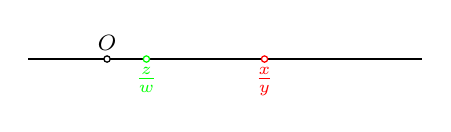
\begin{tikzpicture}
                        % \clip (0,0) rectangle (14.000000,10.000000);
                        {\footnotesize
                        
                        % Drawing segment A B
                        \draw [line width=0.016cm] (1.000000,1.500000) -- (1.960000,1.500000);%
                        \draw [line width=0.016cm] (2.040000,1.500000) -- (2.460000,1.500000);%
                        \draw [line width=0.016cm] (2.540000,1.500000) -- (3.960000,1.500000);%
                        \draw [line width=0.016cm] (4.040000,1.500000) -- (6.000000,1.500000);%
                        
                        % Marking point O by circle
                        \draw [line width=0.016cm] (2.000000,1.500000) circle (0.040000);%
                        \draw (2.000000,1.500000) node [anchor=south] { $O$ };%
                        
                        % Changing color 255 0 0
                        \definecolor{r255g0b0}{rgb}{1.000000,0.000000,0.000000}%
                        \color{r255g0b0}% 
                        
                        % Marking point \frac{x}{y} by circle
                        \draw [line width=0.016cm] (4.000000,1.500000) circle (0.040000);%
                        \draw (4.000000,1.500000) node [anchor=north] { $\frac{x}{y}$ };%
                        
                        % Changing color 0 255 0
                        \definecolor{r0g255b0}{rgb}{0.000000,1.000000,0.000000}%
                        \color{r0g255b0}% 
                        
                        % Marking point \frac{z}{w} by circle
                        \draw [line width=0.016cm] (2.500000,1.500000) circle (0.040000);%
                        \draw (2.500000,1.500000) node [anchor=north] { $\frac{z}{w}$ };%
                        \color{black}
                        }
                    \end{tikzpicture}
                \end{figure}    
    

                Slike pozitivnih racionalnih števil ležijo desno, slike negativnih racionalnih števil pa levo od koordinatnega izhodišča.
                    \begin{figure}[H]
                        \centering
                        \begin{tikzpicture}
                            
                            % \clip (0,0) rectangle (14.000000,10.000000);
                            {\footnotesize
                            
                            % Drawing segment A B
                            \draw [line width=0.016cm] (1.000000,1.500000) -- (3.460000,1.500000);%
                            \draw [line width=0.016cm] (3.540000,1.500000) -- (6.000000,1.500000);%
                            
                            % Changing color 255 0 0
                            \definecolor{r255g0b0}{rgb}{1.000000,0.000000,0.000000}%
                            \color{r255g0b0}% 
                            
                            % Drawing segment B O
                            \draw [line width=0.016cm] (6.000000,1.500000) -- (3.540000,1.500000);%
                            
                            % Marking point pozitivna_tevila
                            \draw (4.750000,1.500000) node [anchor=north] { $pozitivna~ števila$ };%
                            \draw (4.750000,1.500000) node [anchor=south] { $\mathbb{Q}^+$ };%
                            
                            % Changing color 0 255 0
                            \definecolor{r0g255b0}{rgb}{0.000000,1.000000,0.000000}%
                            \color{r0g255b0}% 
                            
                            % Drawing segment O A
                            \draw [line width=0.016cm] (3.460000,1.500000) -- (1.000000,1.500000);%
                            
                            % Marking point negativna_tevila
                            \draw (2.250000,1.500000) node [anchor=north] { $negativna~ števila$ };%
                            \draw (2.250000,1.500000) node [anchor=south] { $\mathbb{Q}^-$ };%
                            
                            % Changing color 0 0 0
                            \definecolor{r0g0b0}{rgb}{0.000000,0.000000,0.000000}%
                            \color{r0g0b0}% 
                            
                            % Marking point O by circle
                            \draw [line width=0.032cm] (3.500000,1.500000) circle (0.040000);%
                            \draw (3.500000,1.500000) node [anchor=south] { $O$ };%
                            \color{black}
                            }
                        \end{tikzpicture}
                    \end{figure}

                    

                    V množici ulomkov velja, da je vsak negativen ulomek manjši od vsakega pozitivnega ulomka.


                    ~

                    Množica racionalnih števil je \textbf{linearno urejena} z relacijo \textit{biti manjši ali enak} ($\leq$) oziroma \textit{biti večji ali enak} ($\geq$). 
                    
                    Za to relacijo linearne urejenosti veljajo naslednje lastnosti:

                    \begin{itemize}
                        \item \textbf{refleksivnost}: $\forall \dfrac{x}{y}\in\mathbb{Q}: \dfrac{x}{y}\leq\dfrac{x}{y}$;
                        \item \textbf{antisimetričnost}: $\forall \dfrac{x}{y},\dfrac{z}{w}\in\mathbb{Q}: \dfrac{x}{y}\leq\dfrac{z}{w}  \land \dfrac{z}{w}\leq\dfrac{x}{y} \Rightarrow \dfrac{x}{y}=\dfrac{z}{w}$;
                        \item \textbf{tranzitivnost}: $\forall \dfrac{x}{y},\dfrac{z}{w},\dfrac{r}{q}\in\mathbb{Q}: \dfrac{x}{y}\leq\dfrac{z}{w}  \land \dfrac{z}{w}\leq\dfrac{r}{q} \Rightarrow \dfrac{x}{y}\leq\dfrac{r}{q}$ in 
                        \item \textbf{stroga sovisnost}: $\forall \dfrac{x}{y},\dfrac{z}{w}\in\mathbb{Q}: \dfrac{x}{y}\leq\dfrac{z}{w}  \lor \dfrac{z}{w}\leq\dfrac{x}{y}$.
                    \end{itemize}
    


                    Množica racionalnih števil pa je tudi \textbf{delno urejena}, in sicer z relacijo \textit{biti manjši} ($<$) oziroma \textit{biti večji} ($>$). 
                
                    Tedaj veljajo le lastnosti: \textbf{refleksivnost}, \textbf{antisimetričnost} in \textbf{tranzitivnost}.


                    
                    ~
            
               
                    Če na obeh straneh neenakosti prištejemo isto število, se neenakost ohrani.
                    $$ \dfrac{x}{y}<\dfrac{z}{w} \quad \Rightarrow \quad \dfrac{x}{y}+\dfrac{r}{q}<\dfrac{z}{w}+\dfrac{r}{q} $$

                    
                    

                    Pri množenju neenakosti s pozitivnim številom se znak neenakosti ohrani.
                    $$ \dfrac{x}{y}<\dfrac{z}{w} \quad \wedge \quad \dfrac{r}{q}>0 \quad \Rightarrow \quad \dfrac{x}{y}\cdot\dfrac{r}{q}<\dfrac{z}{w}\cdot\dfrac{r}{q} $$

                    

                    Pri množenju neenakosti s negativnim številom se znak neenakosti obrne.
                    $$ \dfrac{x}{y}<\dfrac{z}{w} \quad \wedge \quad \dfrac{r}{q}<0 \quad \Rightarrow \quad \dfrac{x}{y}\cdot\dfrac{r}{q}>\dfrac{z}{w}\cdot\dfrac{r}{q} $$

                    

                    %%% naloge
                    ~
                    \begin{naloga}
                        Kateri od ulomkov je večji?
                        \begin{itemize}
                            \item $\frac{3}{7}$, $\frac{3}{8}$ 
                            \item $\frac{7}{3}$, $\frac{8}{3}$ 
                            \item $\frac{2}{5}$, $\frac{3}{10}$ 
                            \item $\frac{1}{100}$, $\frac{1}{200}$ 
                        \end{itemize}
                    \end{naloga}
        
                    \begin{naloga}
                        Katero število je za $\frac{3}{5}$ večje od $\frac{2}{3}$?
                        
                    \end{naloga}
        
                    \begin{naloga}
                        Katero število je za $\frac{1}{3}$ manjše od $\frac{7}{9}$?
                        
                    \end{naloga}
        
                    \begin{naloga}
                        Ulomke uredite po velikosti od večjega k manjšemu.
                        \begin{itemize}
                            \item $\frac{2}{5}$, $\frac{3}{10}$, $\frac{8}{9}$ in $\frac{7}{8}$ 
                            \item $-\frac{1}{2}$, $\frac{-1}{3}$, $\frac{-3}{4}$ in $\frac{2}{-5}$ 
                        \end{itemize}
                    \end{naloga}
        
        
                    \begin{naloga}
                        Ali obstajajo ulomki z imenovalcem $25$, ki so med $\frac{4}{9}$ in $\frac{5}{9}$? Če obstajajo, jih zapišite.
                        
                    \end{naloga}
        
                    \begin{naloga}
                        Ali obstajajo ulomki z imenovalcem $100$, ki so med $\frac{13}{53}$ in $\frac{14}{53}$? Če obstajajo, jih zapišite.
                        
                    \end{naloga}
        
        

                    
    \newpage
    %%% Potence s celimi eksponenti

    \section{Potence s celimi eksponenti}

            Naravna števila so enaka pozitivnim celim številom, torej so potence s pozitivnimi celimi eksponenti enake potencam z naravnimi eksponenti.

            ~

            Potenca z eksponentom enakim $0$ je definirana kot: 
            $$x^0=\begin{cases}
                1; &x\neq 0; \\
                0; &x=0.
            \end{cases}$$

            ~

            Potenca z negativnim celim eksponentom pa je definirana kot:
            $$x^{-n}=\dfrac{1}{x^n}; \quad x\notin\{0\}, n\in\mathbb{N}.$$

            
        \subsection*{Pravila za računanje s potencami s celimi eksponenti}
            V spodaj zapisanih pravilih upoštevamo realni osnovi $x,y\in\mathbb{R}$ in cele eksponente $m,n\in\mathbb{Z}$.
            \begin{itemize}
                \item $x^n\cdot x^m=x^{n+m}$
                \item $x^n\cdot y^n=(xy)^n$
                \item $\left(x^n\right)^m=x^{nm}$
                \item $x^n:x^m=\dfrac{x^n}{x^m}=x^{n-m}$
                \item $x^n:y^n=\dfrac{x^n}{y^n}=\left(\dfrac{x}{y}\right)^n; \quad y\neq 0$
            \end{itemize}


    %%% naloge
    ~\\
            \begin{naloga}
                Poenostavite.
                \begin{itemize}
                    \item $x^{10}:x^5$ 
                    \item $b^4:b^{-11}$ 
                    \item $y^{-3}:y^2$ 
                \end{itemize}
            \end{naloga}

            \begin{naloga}
                Poenostavite.
                \begin{itemize}
                    \item $\frac{x^3y^{-2}}{x^{-2}y^3}$ 
                    \item $\frac{2^{10}a^4b^{-4}}{2^{-2}a^{-2}b}$ 
                    \item $\frac{3^{10}x^{-12}y^{-20}}{6^{10}x^2y^{-3}}$ 
                \end{itemize}
            \end{naloga}


            \begin{naloga}
                Poenostavite.
                \begin{itemize}
                    \item $\left(\frac{-2^5a^{-4}b^3}{2^{-2}ab^{-2}}\right)^2:\left(-\frac{a^2b^4}{2^3a^{-2}}\right)^3$ 
                    \item $\left(\frac{-3^4x^{-2}y^3}{x^3z^2}\right)^{-4}\cdot\left(\frac{3^5x^2z^{-2}}{y^{-3}}\right)^3$ 
                    \item $-\frac{5^5a^4b^{-3}}{a^{-3}b^2}:\left(-\frac{5^2a^{-2}b}{a^2}\right)^2$ 
                \end{itemize}
            \end{naloga}


            \begin{naloga}
                Poenostavite.
                \begin{itemize}
                    \item $\frac{x^{-2}+x^{-1}}{x^{-3}+x^{-2}}$ 
                    \item $\frac{x^{-1}+x^{-2}+x^{-3}}{x^{-4}-x^{-1}}$ 
                    \item $\frac{1+x^{-2}}{x^{-4}-1}$ 
                    \item $\frac{x^{-2}+x^{-3}}{x^{-3}-x^{-2}}$ 
                \end{itemize}
            \end{naloga}


        
            \begin{naloga}
                Poenostavite.
                \begin{itemize}
                    \item $\frac{3^{n+2}-2\cdot 3^{n-1}}{3^{n-2}+3^n}$ 
                    \item $\frac{5^{2n}+5^{2n-1}-2\cdot 5^{2n+1}}{25^n}$ 
                    \item $\frac{7^{3n-3}+3\cdot 7^{3n-2}-7^{3n-4}}{7^{3n-2}-7^{3n-1}}$ 
                    \item $\frac{2^{n-1}+3\cdot 2^n}{4^n+5\cdot 2^{2n-1}}$ 
                \end{itemize}
            \end{naloga}


            \begin{naloga}
                Napišite brez negativnih eksponentov.
                \begin{itemize}
                    \item $x^{-1}+2x^{-2}$ 
                    \item $1-x^{-1}-x^{-2}$ 
                    \item $\frac{1}{x^{-1}}+x^{-1}$ 
                    \item $\left(\frac{\frac{2}{x^{-2}}}{\left(x^{-2}\right)^{-1}}\right)^{-1}$ 
                \end{itemize}
            \end{naloga}
        

            \begin{naloga}
                Poenostavite.
                \begin{itemize}
                    \item $\left(x-x^{-1}\right)\cdot\left(x^2-1\right)^{-1}$ 
                    \item $\frac{x^{-2}+x^{-1}}{x^{-2}-x^{-1}}-\left(1-x\right)^{-1}$ 
                    \item $\left(\frac{x^{-3}-x^{-1}}{1-x^{-2}}\right)^{-1}+\left(\frac{1}{x}\right)^{-1}$ 
                    \item $\left(x^{-2}-2x^{-1}+1\right)^{-1}-\left(x-1\right)^{-2}$ 
                \end{itemize}
            \end{naloga}


\newpage
%%% Decimalni zapis

\section{Decimalni zapis}

        Vsako racionalno število lahko zapišemo na dva načina:
        \begin{itemize}
            \item z \textbf{ulomkom} in 
            \item z \textbf{decimalnim zapisom}.
        \end{itemize}

        ~

        \textbf{Decimalni zapis} sestavljajo tri komponente:
        \begin{itemize}
            \item \textbf{celi del},
            \item \textbf{decimalna pika} oziroma \textbf{decimalna vejica} in 
            \item \textbf{ulomljeni del}.
        \end{itemize}

        ~

        Decimalni zapis racionalnega števila (zapisanega z ulomkom) dobimo tako, 
        da števec ulomka delimo z njegovim imenovalcem.



        \subsection*{Končen decimalni zapis}
        
        \textbf{Končen decimalni zapis} dobimo pri \textbf{desetiških}/\textbf{decimalnih ulomkih}. 
        
        To so ulomki, katerih imenovalec se lahko razširi na potenco števila $10$, takšni imenovalci so oblike $2^n\cdot 5^m$.

        

        \subsection*{Neskončen periodičen decimalni zapis}
        
        \textbf{Neskončen periodičen decimalni zapis} dobimo pri \textbf{nedesetiških}/\textbf{nedecimalnih ulomkih}. 
        
        To so ulomki, katerih imenovalca ne moremo razširiti na potenco števila $10$.

        ~

        Najmanjšo skupino števk, ki se pri neskončnem periodičnem decimalnem zapisu ponavlja, imenujemo \textbf{perioda}.
        Označujemo jo s črtico nad to skupino števk.

        Glede na število števk, ki v njej nastopajo, določimo njen \textbf{red}.

        

%%% naloge

        ~\\

    \begin{naloga}
        Zapišite z decimalnim zapisom.
        \begin{itemize}
                    \item $\dfrac{3}{8}$ 
                    \item $\dfrac{2}{125}$ 
                    \item $\dfrac{6}{25}$ 
                    \item $\dfrac{5}{6}$ 
                    \item $\dfrac{4}{9}$ 
                    \item $\dfrac{4}{15}$ 
                    \item $\dfrac{1}{7}$ 
                    \item $\dfrac{11}{13}$ 
       \end{itemize}
    \end{naloga}



    \begin{naloga}
        Periodično decimalno število zapišite z okrajšanim ulomkom.
        \begin{itemize}
                    \item $0.\overline{24}$ 
                    \item $0.\overline{9}$ 
                    \item $1.\overline{2}$ 
                    \item $1.0\overline{3}$ 
                    \item $1.00\overline{12}$ 
        \end{itemize}
    \end{naloga}

    


    \begin{naloga}
        Izračunajte.
        \begin{itemize}
                    \item $2.3+4.8$ 
                    \item $11.3+2.35$ 
                    \item $0.94+0.24$ 
                    \item $5.6-2.9$ 
                    \item $0.2-1.25$ 
                    \item $12.5-20.61$ 
        \end{itemize}
    \end{naloga}

    


    \begin{naloga}
        Izračunajte.
        \begin{itemize}
                    \item $0.1\cdot 2.44$ 
                    \item $1.2\cdot 0.4$ 
                    \item $11\cdot 0.002$ 
                    \item $0.5\cdot 0.04$ 
                    \item $0.3: 5$ 
                    \item $12.5: 0.05$ 
                    \item $2: 0.02$ 
                    \item $0.15: 0.3$ 
        \end{itemize}
    \end{naloga}

    


    \begin{naloga}
        Izračunajte.
        \begin{itemize}
                    \item $\left(0.24 + 0.06\right):5 - 1.2$ 
                    \item $12:\left(1.2- 0.2\cdot 3\right)+1.2$ 
                    \item $\left(2-0.3:\left(0.025 + 0.035\right)\right)\cdot 0.11$ 
                    \item $\left(1-0.2:\left(0.03+0.02\right)\right)\cdot 1.5$ 
                    \item $0.3\cdot\left(1.2-0.6\cdot\left(0.04+0.06\right)\right)$ 
        \end{itemize}
    \end{naloga}

    